
\documentclass[runningheads]{llncs}
%
\usepackage{amsmath}
\usepackage{amssymb}
\usepackage{amsthm}
\usepackage{multirow}
\usepackage{tikz}
\usepackage{comment}
\usepackage{dsfont}

\usepackage{graphicx}



% Used for displaying a sample figure. If possible, figure files should
% be included in EPS format.
%
% If you use the hyperref package, please uncomment the following line
% to display URLs in blue roman font according to Springer's eBook style:
% \renewcommand\UrlFont{\color{blue}\rmfamily}

\begin{document}
%
%\title{Contribution Title\thanks{Supported by organization x.}}
\title{Learning Temporal Planning Models from Partial Observability by using Constraint Programming\thanks{Supported by organization x.}}

% On the Application of Constraint Programming to Learning and Validating
%
\titlerunning{Learning Temporal Planning Models}
% If the paper title is too long for the running head, you can set
% an abbreviated paper title here
%
\author{Antonio Garrido\inst{1} \and
Sergio Jim\'enez\inst{1}}
%
\authorrunning{A. Garrido, S. Jim\'enez}
% First names are abbreviated in the running head.
% If there are more than two authors, 'et al.' is used.
%
\institute{Universitat Polit\`ecnica de Val\`encia, Camino de Vera s/n. 46022 Valencia, Spain
\email{\{agarridot,serjice\}@dsic.upv.es}}
%
\maketitle              % typeset the header of the contribution
%
\begin{abstract}

The paper shows that existing CSP compilations for temporal planning can be adapted to build action models for temporal planning.


150--250 words.

\keywords{First keyword  \and Second keyword \and Another keyword.}
\end{abstract}
%
%
%
\section{Introduction}
\label{sec:introduction}
{\em Automated Planning} is the model-based approach for the task of selecting actions that achieve a given set of goals. {\em Classical planning} is the vanilla model for automated planning. This planning model assumes: fully observable states, actions with deterministic and instant effects and, goals that are exclusively referred to the last state reached by a plan~\cite{geffner2013concise}.

Besides {\em classical planning}, there is a bunch of more expressive planning models that relax the previous assumptions to compute more detailed solutions than classical plans~\cite{ghallab2004automated}. {\em Temporal planning} is one of these models since it relaxes the {\em instant effects} assumption to compute plans that indicate the precise time-stamp where actions start and end. Actions in {\em temporal planning} have then duration and can be applied in parallel and overlap~\cite{cushing2007temporal}.

Despite the potential of automated planning, state-of-the-art planners compute plans of several hundreds of actions in seconds time~\cite{vallati20152014}, its applicability to real-world tasks is still limited because of the complexity of specifying correct and complete planning models. The more expressive the planning model, the more evident becomes this {\em knowledge acquisition bottleneck}.

In this paper we show that existing CSP compilations for temporal planning can be adapted to build temporal planning models with regard to observations of plan executions. The work assumes that, despite the aimed temporal action model is unknown, there is {\em partial observability} of the execution of temporal plans computed with that model and, that such observations are {\em noiseless} (meaning that if the value of a fluent is observed, then the observation is correct).



\section{Background}
\label{sec:background}
This section formalizes the planning models that we use in the paper ({\em classical} and {\em temporal planning}) as well as the {\em Constraint Satisfaction Problem}, the technique we leverage to improve the expressiveness of a given classical planning model.

\subsection{Classical Planning}
We use $F$ to denote the set of {\em fluents} (propositional variables) describing a state. A {\em literal} $l$ is a valuation of a fluent $f\in F$; i.e. either~$l=f$ or $l=\neg f$. A set of literals $L$ represents a partial assignment of values to fluents (without loss of generality, we will assume that $L$ does not contain conflicting values). Given $L$, let $\neg L=\{\neg l:l\in L\}$ be its complement. We use $\mathcal{L}(F)$ to denote the set of all literal sets on $F$; i.e.~all partial assignments of values to fluents. A {\em state} $s$ is a full assignment of values to fluents; $|s|=|F|$.

Each classical planning action $a\in A$ has a precondition $\pre(a)\in\mathcal{L}(F)$ and a set of effects $\eff(a)\in\mathcal{L}(F)$. The semantics of actions $a\in A$ is specified with two functions: $\rho(s,a)$ denotes whether action $a$ is {\em applicable} in a state $s$ and $\theta(s,a)$ denotes the {\em successor state} that results of applying action $a$ in a state $s$. Then, $\rho(s,a)$ holds iff $\pre(a)\subseteq s$, i.e.~if its precondition holds in $s$. The result of executing an applicable action $a\in A$ in a state $s$ is a new state $\theta(s,a)=(s\setminus \neg\eff(a))\cup\eff(a)$. Subtracting the complement of $\eff(a)$ from $s$ ensures that $\theta(s,a)$ remains a well-defined state. The subset of action effects that assign a positive value to a state fluent is called {\em positive effects} and denoted by $\eff^+(a)\in \eff(a)$ while $\eff^-(a)\in \eff(a)$ denotes the {\em negative effects} of an action $a\in A$.

We assume that actions $a\in A$ are instantiated from given action schemas, as in PDDL. Figure~\ref{fig:flyc} shows the {\em fly} action schema from the {\em zenotravel} domain encoded in PDDL2.1~\cite{fox2003pddl2}. According to this action model an {\em aircraft} moves from one {\em city} to another consuming a single unit of {\em fuel}.

A {\em classical planning problem} is a tuple $P=\tup{F,A,I,G}$, where $I$ is an initial state and $G\in\mathcal{L}(F)$ is a goal condition. A {\em sequential plan} is an action sequence $\pi=\tup{a_1, \ldots, a_n}$ whose execution induces the {\em state trajectory} $\tau=\tup{s_0, s_1, \ldots, s_n}$ such that $s_0=I$ and, for each {\small $1\leq i\leq n$}, $a_i$ is applicable in $s_{i-1}$ and generates the successor state $s_i=\theta(s_{i-1},a_i)$. The {\em plan length} is denoted with $|\pi|=n$ . A plan $\pi$ {\em solves} $P$ iff $G\subseteq s_n$, i.e.,~if the goal condition is satisfied at the last state reached after following the application of the plan $\pi$ in the initial state $I$. A solution plan for $P$ is {\em optimal} if it has minimum length.

\begin{figure}
	\begin{scriptsize}
		\begin{verbatim}
(:action fly
 :parameters (?a - aircraft ?c1 ?c2 - city ?l1 ?l2 - flevel)
 :precondition (and (at ?a ?c1) (fuel-level ?a ?l1)
                    (next ?l2 ?l1))
 :effect (and (not (at ?a ?c1)) (at ?a ?c2)
              (not (fuel-level ?a ?l1))
              (fuel-level ?a ?l2)))
		\end{verbatim}
	\end{scriptsize}
	\caption{PDDL1.1 encoding of the classical action model of the {\em fly} operator from the {\em zenotravel} domain.}
	\label{fig:flyc}
\end{figure}


\subsection{Temporal Planning}
A {\em temporal planning problem} is a tuple $P=\tup{F,A,I,G}$, where the set of fluents $F$, the initial state $I$, and the goal conditions $G\subseteq\mathcal{L}(F)$ are defined as in a {\em classical planning problem}. However, $A$ represents here a set of {\em durative actions} such that each $a\in A$ is now defined as follows:
\begin{itemize}
\item $d(a)$, a scalar indicating the action duration.
\item $\cond_s(a)\subseteq\mathcal{L}(F)$, $\cond_o(a)\subseteq\mathcal{L}(F)$ and $\cond_e(a)\subseteq\mathcal{L}(F)$, that respectively represent the {\em conditions} (literals that must hold for the action $a$ to be applicable) {\em at start}, {\em over all}, and {\em at end} of the action.

\item $\add_s(a)\subseteq\mathcal{L}(F)$ and $\add_e(a)\subseteq\mathcal{L}(F)$, that are the {\em positive effects} (fluents set to true by the application of $a$) {\em at start} and {\em at end} of the action application.
\item  $\del_s(a)\subseteq\mathcal{L}(F)$ and $\del_e(a)\subseteq\mathcal{L}(F)$, that are the {\em negative effects} (also {\em at start} and {\em at end}).
\end{itemize}

Figure~\ref{fig:flyt} shows the {\em durative} version of the {\em fly} schema from the {\em zenotravel} domain encoded in PDDL2.1~\cite{fox2003pddl2}. Despite {\em durative actions} are not longer instantaneous (they have a duration), conditions {\em at start} and {\em at end} are checked instantaneously. In the same way, {\em at start} and {\em at end} effects are instantaneously applied (effects can only happen {\em at start} or {\em at end} since continuous effects are not considered). With this regard, the semantics of a {\em durative action} $a\in A$ can be defined in terms of two discrete events $start_a$ and $end_a$. The duration imposes that $end_a$ must occur exactly $d(a)$ time units after $start_a$ and {\em over all} conditions of $a$ must hold at any state between $start_a$ and $end_a$.

A {\em temporal plan} is a set of pairs $\pi=\tup{(a_1,t_1), \ldots, (a_n,t_n)}$ such that each pair contains a {\em durative} action $a\in A$ and its scheduled {\em start time}. Note that each $(a,t_a)\in \pi$ pair induces two discrete events, $start_a$ and $end_a$ with associated time-stamps $t$ and $t+d(a)$. If we order the $2n$ events induced from $\pi$ by their associated times, we obtain the {\em event sequence}, $E_{\pi}=\langle e_1,\ldots,e_m\rangle$, where {\small $1\leq m\leq 2n$}. Each $e_i$, {\small $1\leq i\leq m$}, is a {\em joint event} composed of one or more individual events of $\pi$ that all have the same associated time. We say that $\pi$ has {\em simultaneous events} if $m<2n$, i.e.~if at least one joint event is composed of multiple individual events.

The {\em execution} of a temporal plan $\pi$ starting from $I$, induces the {\em state trajectory} $\tau=\tup{s_0, s_1, \ldots, s_m}$ such that $s_0=I$ and $a_i$ ({\small $1\leq i\leq m$}) is a classical planning action modeling the corresponding {\em joint event} $e_i$ and satisfying that $a_i$ is applicable in $s_{i-1}$ and that the application of $a_i$ generates the successor state $s_i=\theta(s_{i-1},a_i)$~\cite{jimenez2015temporal}. A {\em temporal plan} $\pi$ is a solution for $P$ iff the last state reached by its execution starting from $I$ satisfies that $G\subseteq s_m$.

The quality of a temporal plan is given by its {\em makespan}, i.e. the temporal duration from the the start of the first temporal action to the end of the last temporal action. Without loss of generality, we assume that the first temporal action is scheduled to start at time 0, i.e. $min_{\tup{a,t_a}\in\pi}= 0$. In this case, the makespan of a temporal plan $\pi$ is formally defined as $max_{\tup{a,t_a}\in\pi}(t_a+d(a))$. A temporal plan $\pi$ is {\em optimal} for a given temporal planning proble $P$ iff its makespan is minimal.

Figure~\ref{fig:plan} shows an example of a temporal plan for solving a problem from the {\em zenotravel domain}.

\begin{figure}
	\begin{scriptsize}
		\begin{verbatim}
(:durative-action fly
 :parameters (?a - aircraft ?c1 ?c2 - city ?l1 ?l2 - flevel)
 :duration (= ?duration 180)
 :condition (and (at start (at ?a ?c1))
                 (at start (fuel-level ?a ?l1))
                 (at start (next ?l2 ?l1)))
 :effect (and (at start (not (at ?a ?c1)))
              (at end (at ?a ?c2))
              (at end (not (fuel-level ?a ?l1)))
              (at end (fuel-level ?a ?l2))))
		\end{verbatim}
	\end{scriptsize}
	\caption{PDDL2.1 {\em durative} encoding of the {\em fly} schema from the {\em zenotravel} domain.}
	\label{fig:flyt}
\end{figure}


\begin{figure}
        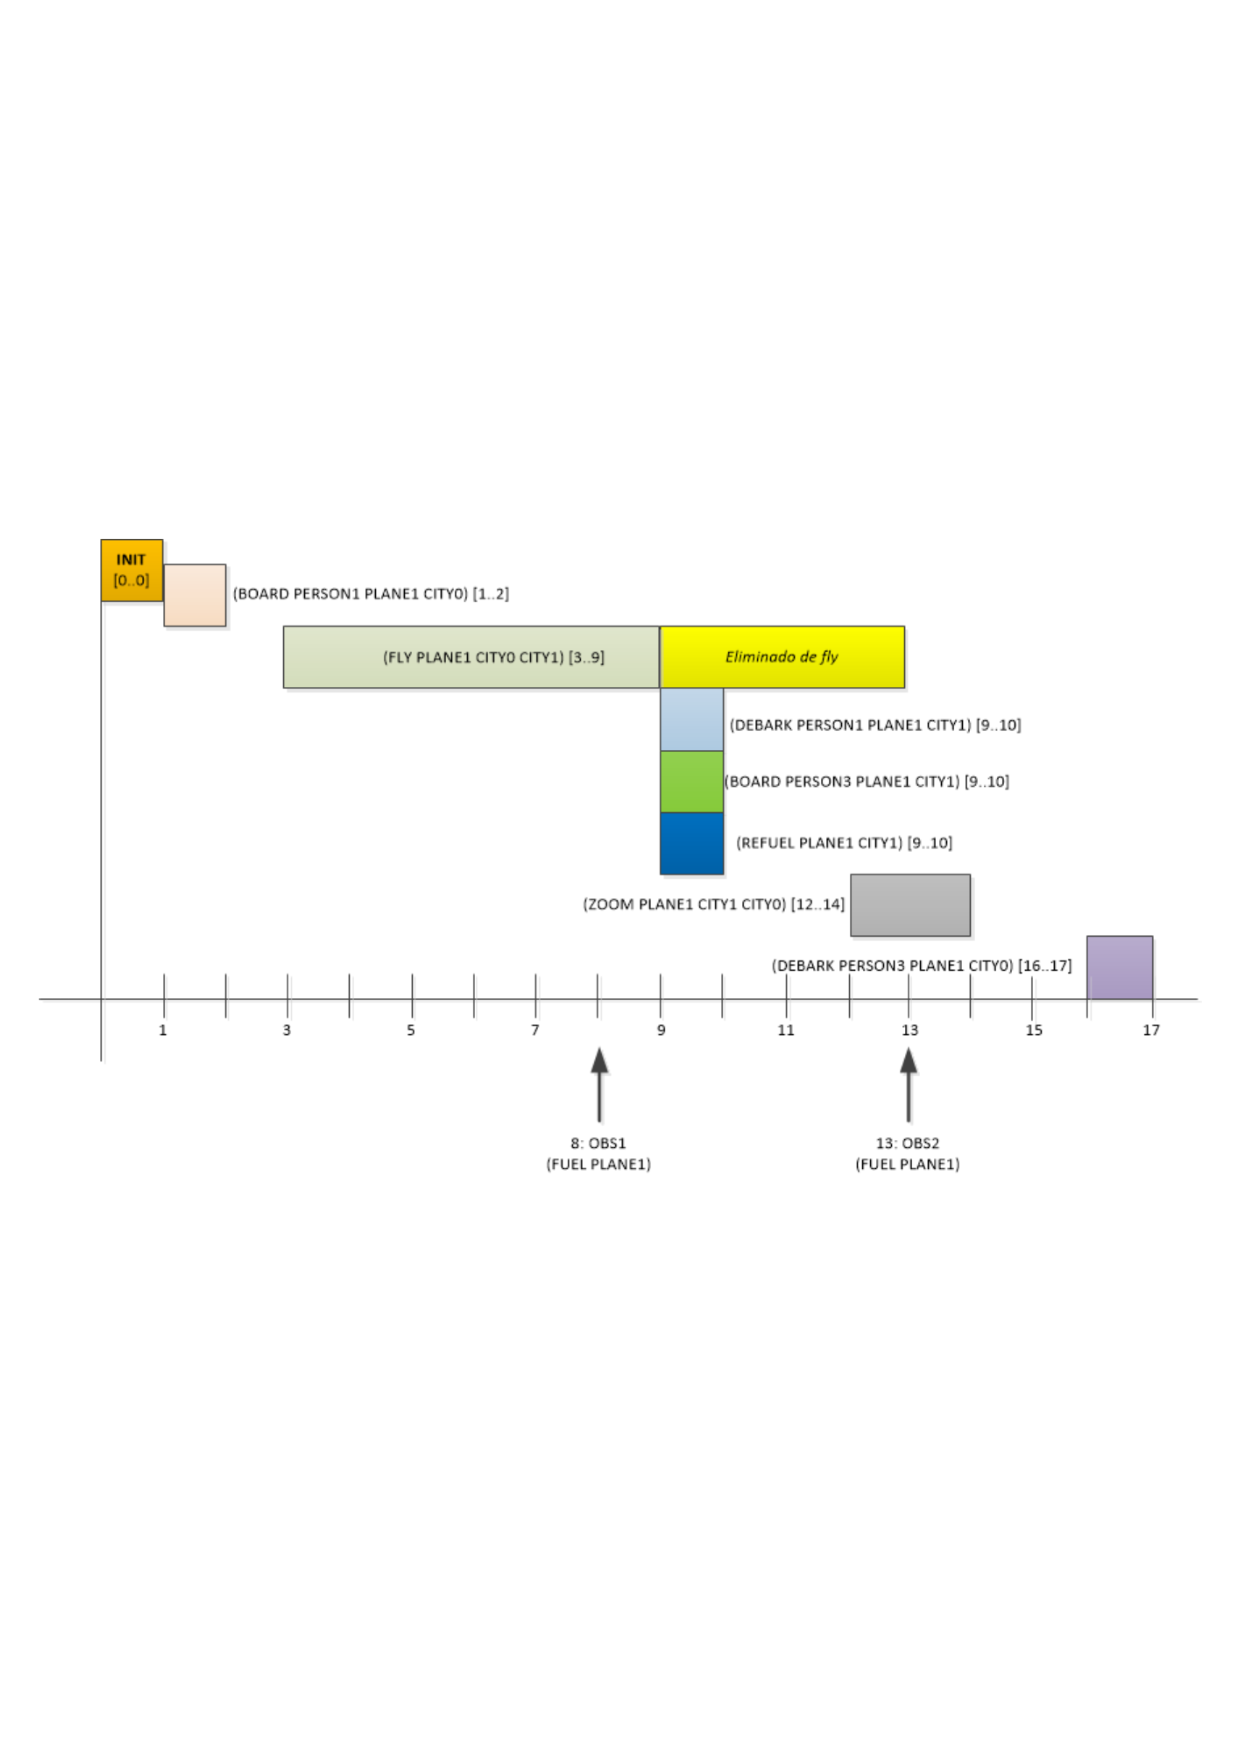
\includegraphics[width=0.5\textwidth]{plan}
	\caption{Example of a temporal plan for solving a problem from the {\em zenotravel domain}.}
	\label{fig:plan}
\end{figure}


\subsection{The observation model}
The work assumes that, despite the aimed temporal action model is unknown, there is {\em partial observability} of the execution of temporal plans computed with that model and, that such observations are {\em noiseless} (meaning that if the value of a fluent is observed, then the observation is correct).

In more detail, given a {\em temporal planning problem} $P=\tup{F,A[\cdot],I,G}$ (where the action model that defines the semantics of the actions in $A[\cdot]$ is unknown), and a temporal plan $\pi$ s.t. $\pi$ solves $P$ and such that it induces the state trajectory $\tau=\tup{s_0, s_1, \ldots, s_m}$. The {\em observation} of that trajectory is denoted by $obs(\tau)$ and it defines the same sequence of states induced by the execution of $\pi$ on $P$ but where the value of certain fluents may be omitted, i.e.~$|s^o_i|\leq |F|$ for every $s^o_i\in obs(\tau)$. Each state observation is labeled with its corresponding time-stamp $i$.

\begin{definition}[Explaning an observation]
Given a {\em temporal planning problem} $P$ and a sequence of partially observed states $\mathcal{O}(\tau)$, we say that a plan $\pi$ {\em explains the observation} (denoted $\pi\mapsto\mathcal{O}(\tau)$) iff $\pi$ is a solution for $P$ that is {\em  consistent} with $\mathcal{O}(\tau)$. If $\pi$ is also optimal, we say that $\pi$ is the {\em best explanation} for $\mathcal{O}(\tau)$.
\end{definition}

Given a {\em temporal planning problem} $P=\tup{F,A,I,G}$, we say that an action model $\mathcal{M}$ is a definition of the $\tup{\rho,\theta}$ functions of every action in $A$. Further we say that a model $\mathcal{M}$ {\em explains} a sequence of observations $\mathcal{O}(\tau)$ iff, when the $\tup{\rho,\theta}$ functions of the actions in $P$ are given by $\mathcal{M}$, there exists a solution plan for $P$ that explains $\mathcal{O}(\tau)$.


\subsection{Constraint Satisfaction Problem}
A {\em Constraint Satisfaction Problem} is defined as the triple $\tup{X,D,C}$ where:
\begin{itemize}
\item $X=\tup{x_0, \ldots, x_n}$ is a set of $n$ finite domain variables.
\item $D=\tup{D_{x_0}, \ldots, D_{x_n}}$ are the respective domains defining the set of possible values for each variable $x\in X$.
\item $C=\tup{c_0, \ldots, c_m}$ is a set of constraints bounding the possible values of the variables in $X$. Every constraint $c\in C$, is in turn a pair $c=(X_c,r_c)$ where:
\begin{itemize}
\item $X_c\subseteq X$ is a subset of $k\leq n$ variables.
\item $r_c$ is a $k$-ary relation on the corresponding subset of domains.
\end{itemize}
\end{itemize}

An {\em evaluation} of the variables is a function from a subset of variables to a particular set of values in the corresponding subset of domains. An evaluation $v$ {\em satisfies} a constraint $c=(X_c,r_c)$ if the values assigned to the variables in $X_c$ satisfy the relation $r_c$. An evaluation of $X$ is {\em consistent} if it does not violate any of the constraints in $C$. An evaluation is {\em complete} if it includes values for all the variables. An evaluation is a {\em solution} for a given CSP $\tup{X,D,C}$ if it is both {\em consistent} and {\em complete}.

\section{Building Temporal Planning Models with Constraint Programming}
\label{sec:learning}
This section details our approach for building temporal planning models from the {\em observation of plan executions} and using {\em constraint programming}.

\subsection{The space of temporal action models}
We assume that the durative actions $a\in A$ of a temporal planning problem $P$ are instantiated from given action schemas, as in PDDL. The space of possible models for a {\em durative action schema} $\xi$ is then given by $\Psi$ (the set of {\em predicates} that shape the propositional state variables) and the list of {\em parameters} of that schema, $pars(\xi)$.

With this regard, we denote the set of FOL interpretations of $\Psi$ over the parameters $pars(\xi)$ as ${\mathcal I}_{\Psi,\xi}$ (for domains that allow object typing in the predicates, the FOL interpretations also requires that objects and parameters share the same type). For instance, in the {\em zenotravel} domain the ${\mathcal I}_{\Psi,\xi}$ set contains eight elements for the {\small\tt fly} schemata, ${\mathcal I}_{\Psi,fly}$={\small\tt\{at($a,c_1$), at($a,c_2$), next($l_1,l_1$), next($l_1,l_2$), next($l_2,l_1$), next($l_2,l_2$), fuel-level($a,l_1$), fuel-level($a,l_2$)\}}.

Despite any element of ${\mathcal I}_{\Psi,\xi}$ can {\em a priori} appear in the {\em conditions} and {\em effects} of schema $\xi$, the space of possible durative schemata is bounded by constraints of three kinds:
\begin{enumerate}
\item {\em Syntactic constraints}. We require $del_s(\xi)\subseteq cond_s(\xi)$, $del_s(\xi)\cap add_s(\xi)=\emptyset$ and $cond_s(\xi)\cap add_s(\xi)=\emptyset$ as well as the equivalent constraints for the {\em at end} time-stamp (similar syntactic constraints are usually imposed to \strips\ schemes). Considering exclusively these syntactic constraints, the size of the space of possible {\em durative} schemata is given by $2^{5\times|{\mathcal I}_{\Psi,\xi}|}$.
\item {\em Domain-specific constraints}. One can introduce domain-specific knowledge to constrain further the space of possible schemata. For instance, in the {\em zenotravel} domain one can argue that {\small\tt next($l_1$,$l_1$)} and {\small\tt next($l_2$,$l_2$)} will not appear in the {\em conditions} or {\em effects} of an action schema $\xi$ because, in this specific domain, the {\tt\small next} predicate codes the {\em successor} function for {\em natural numbers}. As a rule of thumb, {\it state invariants} constraining the possible states of a given planning domain belong to this second class of constraints~\cite{fox:TIM:JAIR1998}.

\item {\em Observation constraints}. A sequence of state observations $\mathcal{O}(\tau)$ depicts {\em semantic knowledge} that constraints further the space of possible action schemata.
\end{enumerate}

\subsection{The modeling task}
The task of building a temporal planning model from the observation of a plan execution is formalized as $\Lambda=\tup{P,M,obs(\tau)}$:
\begin{itemize}
\item $P=\tup{F,A[\cdot],I,G}$ is a temporal planning problem where $A[\cdot]$ is a set of actions. For each $a\in A[\cdot]$, the semantics of $a$ is unknown; i.e. the functions $\rho$ and/or $\theta$ of $a$ are undefined.
\item $M=\{\mathcal{M}_1,\ldots,\mathcal{M}_k\}$ is a set of {\em k different planning models} for the actions in $A[\cdot]$. A model $\mathcal{M}\in M$ defines the semantics of every action in $A[\cdot]$. Planning models differ in the $\tup{\rho,\theta}$ functions of the actions but they all use the same set of state variables $F$.
\item $obs(\tau)$ is a sequence of partial states that corresponds to a noiseless observation of the actual temporal plan execution such that $s_0\in obs(\tau)$ is a {\em fully observed} state. More precisely, $s_0=I$ and $|s_0|=|F|$. This means that the set of predicates and objects that shape the fluents of the temporal plannin problem are inferrable from $s_0$.
\end{itemize}

A {\em solution} to a learning task $\Lambda=\tup{P,obs(\tau)}$ is a temporal action model $\mathcal{M}\in M$ that {\em explains} the input observation $obs(\tau)$.

\subsection{A CSP for computing temporal action models}
Given a $\Lambda=\tup{P,M,obs(\tau)}$ task for building a {\em temporal planning} model, then we define a compilation that outputs the following $\tup{X,D,C}$ CSP:

\subsubsection{Variables.} The set of variables $X$ comprises:
\begin{itemize}
\item For each state observation in $obs(\tau)$:
\begin{itemize}
\item $start_a$, indicating the scheduled time-stamp for the start of the observed action $a$. The domain of this variable is $[t_a]$, i.e. a singleton given by the input observation.
\item $duration_a$ representing the action duration. The domain of this variable is $[0,max_t]$ where $max_t$ is the maximum-time stamp in the input observation $obs(\tau)$.
\item $end_a$ is a derived variable, defined in $\mathds{Z}^+$, that indicates the time-stamp for the end of the observed action $a$. The value of this variable is $end_a = start_a + duration_a$.
\item $preS_{f,a}$ and $preE_{f,a}$ are Boolean variables indicating whether fluent $f$ is a condition ({\em at start} or {\em at end}) of the action $a$ in the input. This set of variables is given by the $M$, the input set of possible models for the planning actions.
\item $support_{f,a_i}$ indicates the action supporter of the fluent $f$ for action $a_i$. The domain of these variables is the set of actions.
\item $time_{f,a}$ is a variable indicating when the value of $f$ is modified by action $a$. The domain of this variable is $[start_a,max_t]$.
\end{itemize}
\end{itemize}

\subsubsection{Constraints.} The domains of the variables in $X$ is bound by the following set $C$ of constraints:
\begin{itemize}
\item For each action $a$ observed in a $\omega$:
\begin{itemize}
\item $end_a = start_a + duration_a$.
\item $time_{f,a_i}\neq time_{\neg f,a_j}$.
\item $time_{f,a}= start_a$ XOR $time_{f,a}= end_a$.
\item $start_a\leq preS_{f,a}\leq preE_{f,a}\leq end_a$.
\item IF $supports_{f,a_i}=a_j$ THEN:
\begin{enumerate}
\item $time_{f,a_i}\textless  preS_{f,a_j}$.
\item $time_{f,a_i}\textless  end_{a_j}$.
\item $time_{f,a_k}\textless time_{f,a_i}$ OR $time_{f,a_k}\textless time_{f,a_j}$.
\end{enumerate}
\item $(start_{a_1} = preS_{f,_{a_1}}$ AND $start_{a_n} = preS_{f,a_{a_n}})$ OR $(end_{a_1} = preS_{f,_{a_1}}$ AND $end_{a_n} = preS_{f,a_{a_n}})$. Constraints of the same kind are also defined for the variables $preE_{f,a}$ and $time_{f,a}$.
\item .
\end{itemize}
\end{itemize}

Given a solution for the CSP output by our compilation, the action model $\mathcal{M}$ that solves $\Lambda=\tup{P,obs(\tau)}$ is computable in linear time and space.


\subsection{Compilation properties}
\begin{lemma}
Soundness. Any solution for the CSP output by our compilation induces a set of action models $\mathcal{M}'$ that solves $\Lambda=\tup{\mathcal{M},\omega}$.
\end{lemma}


\begin{lemma}
Completeness. Any set of action models $\mathcal{M}'$ that solves $\Lambda=\tup{\mathcal{M},\omega}$ is computable solving the CSP output by our compilation.
\end{lemma}




\section{Assessing Temporal Planning Models with Constraint Programming}
An interesting aspect of our compilation approach is that when a single possible input model $M=\{\mathcal{M}\}$ is given in $\Lambda$, the compilation serves to validate whether the observation $obs(\tau)$ follows the given model $\mathcal{M}$:

\begin{itemize}
	\item $\mathcal{M}$ is proved to be a {\em valid} action model for the given input data in $obs(\tau)$ iff a solution for the output CSP can be found.
	\item $\mathcal{M}$ is proved to be a {\em invalid} action model for the given input data $obs(\tau)$ iff the output CSP is unsolvable. This means that $\mathcal{M}$ cannot {\em explain} the given observation of the plan execution.
\end{itemize}

This validation capacity of our compilation is beyond the functionality of VAL (the plan validation tool~\cite{howey2004val}) because our approach is able to address {\em model validation} of a partial (or even an empty) action model with a partially observed plan trace. On the other hand, VAL requires (1) a full plan and (2), a full action model for plan validation.

\section{Experimental evaluation}
\label{sec:evaluation}

\subsection{Starting from a partially specified temporal planning model}
The set $M$ of different possible temporal planning models can be given by an {\em incomplete (annotated) model}~\cite{sreedharan2018handling}. Given a set of fluents $F$ then, a {\em partially specified action model} $M$ is a set of possible models for the actions in $A[\cdot]$ such that: (1), any model $\mathcal{M}\in M$ is a definition of the $\tup{\rho,\theta}$ functions of every action in $A[\cdot]$ and (2), for every $\mathcal{M}\in M$ the $\tup{\rho,\theta}$ functions are defined in the set of state variables $F$. (Note that if $M$ is a singleton it represents a {\em fully specified action model}).

\subsection{Starting from a classical planning model}
In this case the set $M$ of {\em different possible temporal planning models} is given by a classical planning model that bounds conditions and effects to the preconditions and effects that appear in the classical planing model. This task corresponds then to improving the expressiveness of a given classical planing model to build a temporal planning model that is consistent with the observation given as input.





\subsection{Starting from scratch}


\section{Related work}
\label{sec:related}
{\em Boolean satisfiability} (SAT) is a powerful problem solving approach that has shown successful to address challenging classical planning task~\cite{kautz1999unifying,rintanen2009planning,rintanen2012planning}. Likewise {\em Constraint Satisfaction Problems} (CSP) has also been used to synthesize solution plans to numeric and temporal planning problems~\cite{do2001planning,lopez2003generalizing,vidal2006branching,garrido2009constraint}.

\section{Conclusions}
\label{sec:conclusions}
%
% ---- Bibliography ----
%
% BibTeX users should specify bibliography style 'splncs04'.
% References will then be sorted and formatted in the correct style.
%
\bibliographystyle{splncs04}
\bibliography{tmodeling}
%
%\begin{thebibliography}{8}
%\end{thebibliography}
\end{document}



in environments where observed data corresponds to
sequences of activities performed by an agent. Hence, the data provides indirect information
on the agent’s beliefs, actions, goals and/or plans that lead it to carry out those activities. We
hypothesize that we can efficiently build models of those activities to help future decisions.


with
recommendations on future behavior (actions, plans or goals) based on learning models of
their past behavior and recognition of their present actions, plans or goals. In order to achieve
the objective, we will integrate techniques from machine learning, activity/plan recognition and
automated planning.


analyze information from sensors in order to generate diverse models of an
agent’s behavior, such as planning domain models, probabilistic models, or generic classifiers.
These models will allow the recognition system to use diverse methods to predict the plan/action/goal the agent is pursuing and build plans or provide recommendations that assist
humans or software/robotic agents in their daily activities.

helping elders or generic tasks; and traffic management
to help smart cities decision making.


plan and goal recognition. recognize the
activities, plans and/or goals of other agents (human or robots) in order to anticipate their
needs or actions

such as home
automation, where the system will learn about the habits and behaviour of the inhabitants, it
will recognize critical situations and will suggest executing specific actions to avoid criticality
or focus on a different goal. In general, proactive assistant agents



Plan recognition is the process of observing the current actions/behaviour of an agent to predict
its future actions. Goal recognition is a subproblem of plan recognition with the objective of
discovering the terminal goal of an agent given its behaviour



Plan recognition is the process of observing the current actions/behaviour of an agent to predict
its future actions. Goal recognition is a subproblem of plan recognition with the objective of
discovering the terminal goal of an agent given its behaviour


IMPORTANTE: consistent with the sequence of observations, in order to select the hypothesis that best explains the
observations. The intuition behind inverse-planning-based approaches is that, given a sequence of
observations and a set of possible goals, the most likely goal to be pursued by an agent is the one which optimal plan is most consistent with the given observations


learning planning models from partial (incomplete) observability


decision support systems in military operations,
emergency management, e-Health, logistics, tourism, transportation, data-mining or e-learning


Para related work ver: memoria Learning action models (pag 12)



can be used in different real-world applications. We are
interested in environments where observed data is regarded as sequences of activities and
thus provide helpful insight to intelligent assistants (domotics, or robotics for helping aging
people), decision making in smart cities (traffic), suggesting better-valued goals or
recommendation of alternative plans that report higher utility to the users (tourism). In
particular, the key idea is to use the generated models in automated planning, so as to propose
the agent what to do, how to do something or how to do it differently.
